\RequirePackage{fix-cm}
\documentclass[tikz,border=6pt]{standalone}
% Shared style for the model diagrams in this folder.
% Each diagram is a standalone document that loads fix-cm, then
% \documentclass[tikz,border=6pt]{standalone}, then inputs this file.
% scripts/build_diagrams.sh compiles every diagram except this file.
% Adapted from epiforecasts/BVDOutbreakSize docs/diagrams/style.tex.

\usepackage[T1]{fontenc}
\usepackage[scaled=0.95]{helvet}
\renewcommand{\familydefault}{\sfdefault}
\usepackage{amsmath,amssymb}
\usetikzlibrary{arrows.meta,positioning,fit,backgrounds,calc,shapes.misc}

% Palette: one colour per role.
% Latent quantities are blue, observed data orange, fixed inputs taken
% from the data purple, and parameters a neutral grey.
\definecolor{latentfill}{HTML}{E3EEF9}
\definecolor{latentline}{HTML}{2B5C8A}
\definecolor{datafill}{HTML}{FCE9D6}
\definecolor{dataline}{HTML}{B35A12}
\definecolor{jointfill}{HTML}{EEE4F5}
\definecolor{jointline}{HTML}{6A3D9A}
\definecolor{paramfill}{HTML}{F2F2F2}
\definecolor{paramline}{HTML}{6E6E6E}
\definecolor{textgrey}{HTML}{4A4A4A}

\tikzset{
  every node/.style={font=\small, text=black,
    execute at begin node={\thickmuskip=5mu\medmuskip=4mu\thinmuskip=3mu
      \hyphenpenalty=10000\exhyphenpenalty=10000}},
  box/.style={rectangle, rounded corners=3pt, draw, line width=0.8pt,
    align=center, inner sep=5pt, minimum height=9mm},
  latent/.style={box, fill=latentfill, draw=latentline},
  data/.style={box, fill=datafill, draw=dataline},
  joint/.style={box, fill=jointfill, draw=jointline},
  param/.style={box, fill=paramfill, draw=paramline},
  group/.style={rectangle, rounded corners=6pt, draw=#1, line width=0.8pt,
    dashed, inner sep=8pt},
  grouplabel/.style={font=\small\bfseries, text=#1, anchor=south west,
    inner sep=2pt},
  flow/.style={-{Stealth[length=2.6mm,width=2mm]}, line width=0.9pt,
    draw=black!75},
  jointflow/.style={flow, draw=jointline, line width=1.1pt},
  biflow/.style={{Stealth[length=2.4mm,width=1.9mm]}-{Stealth[length=2.4mm,width=1.9mm]},
    line width=0.9pt, draw=latentline},
  edgelabel/.style={font=\footnotesize, text=textgrey, fill=white,
    inner sep=1.5pt, align=center},
  note/.style={font=\footnotesize, text=textgrey, align=left},
  title/.style={font=\normalsize\bfseries, align=center},
  tag/.style={rectangle, rounded corners=2pt, fill=jointline,
    text=white, font=\footnotesize\bfseries, inner sep=2pt},
  keyswatch/.style={rectangle, rounded corners=2pt, line width=0.8pt,
    minimum width=7mm, minimum height=4mm, inner sep=0pt},
}

% Colour key, a row of swatches starting at the coordinate #2 (west end).
% Pass [joint] to add the fixed-input swatch.
\newcommand{\colourkey}[2][]{%
  \node[keyswatch, fill=paramfill, draw=paramline, anchor=west] (k1) at #2 {};
  \node[note, anchor=west] (l1) at (k1.east) {parameter};
  \node[keyswatch, fill=latentfill, draw=latentline, right=3mm of l1] (k2) {};
  \node[note, anchor=west] (l2) at (k2.east) {latent quantity};
  \node[keyswatch, fill=datafill, draw=dataline, right=3mm of l2] (k3) {};
  \node[note, anchor=west] (l3) at (k3.east) {observed data and likelihood};
  \ifx\relax#1\relax\else
    \node[keyswatch, fill=jointfill, draw=jointline, right=3mm of l3] (k4) {};
    \node[note, anchor=west] (l4) at (k4.east) {fixed input from the data};
  \fi
}

% The smallest text size. The figures are scaled to the page column, about
% 1.5 times their natural width, so 8.5 pt renders at about 12.5 px.
\renewcommand{\footnotesize}{\fontsize{8.5}{10.2}\selectfont}


% The province renewal model (hubrenewal) as a generative chain:
% parameters, the coupled renewal, confirmed onsets, the onset-to-report
% delay and missingness, and the hub's observation streams. Maths follows
% docs/methods/model.md.

\begin{document}
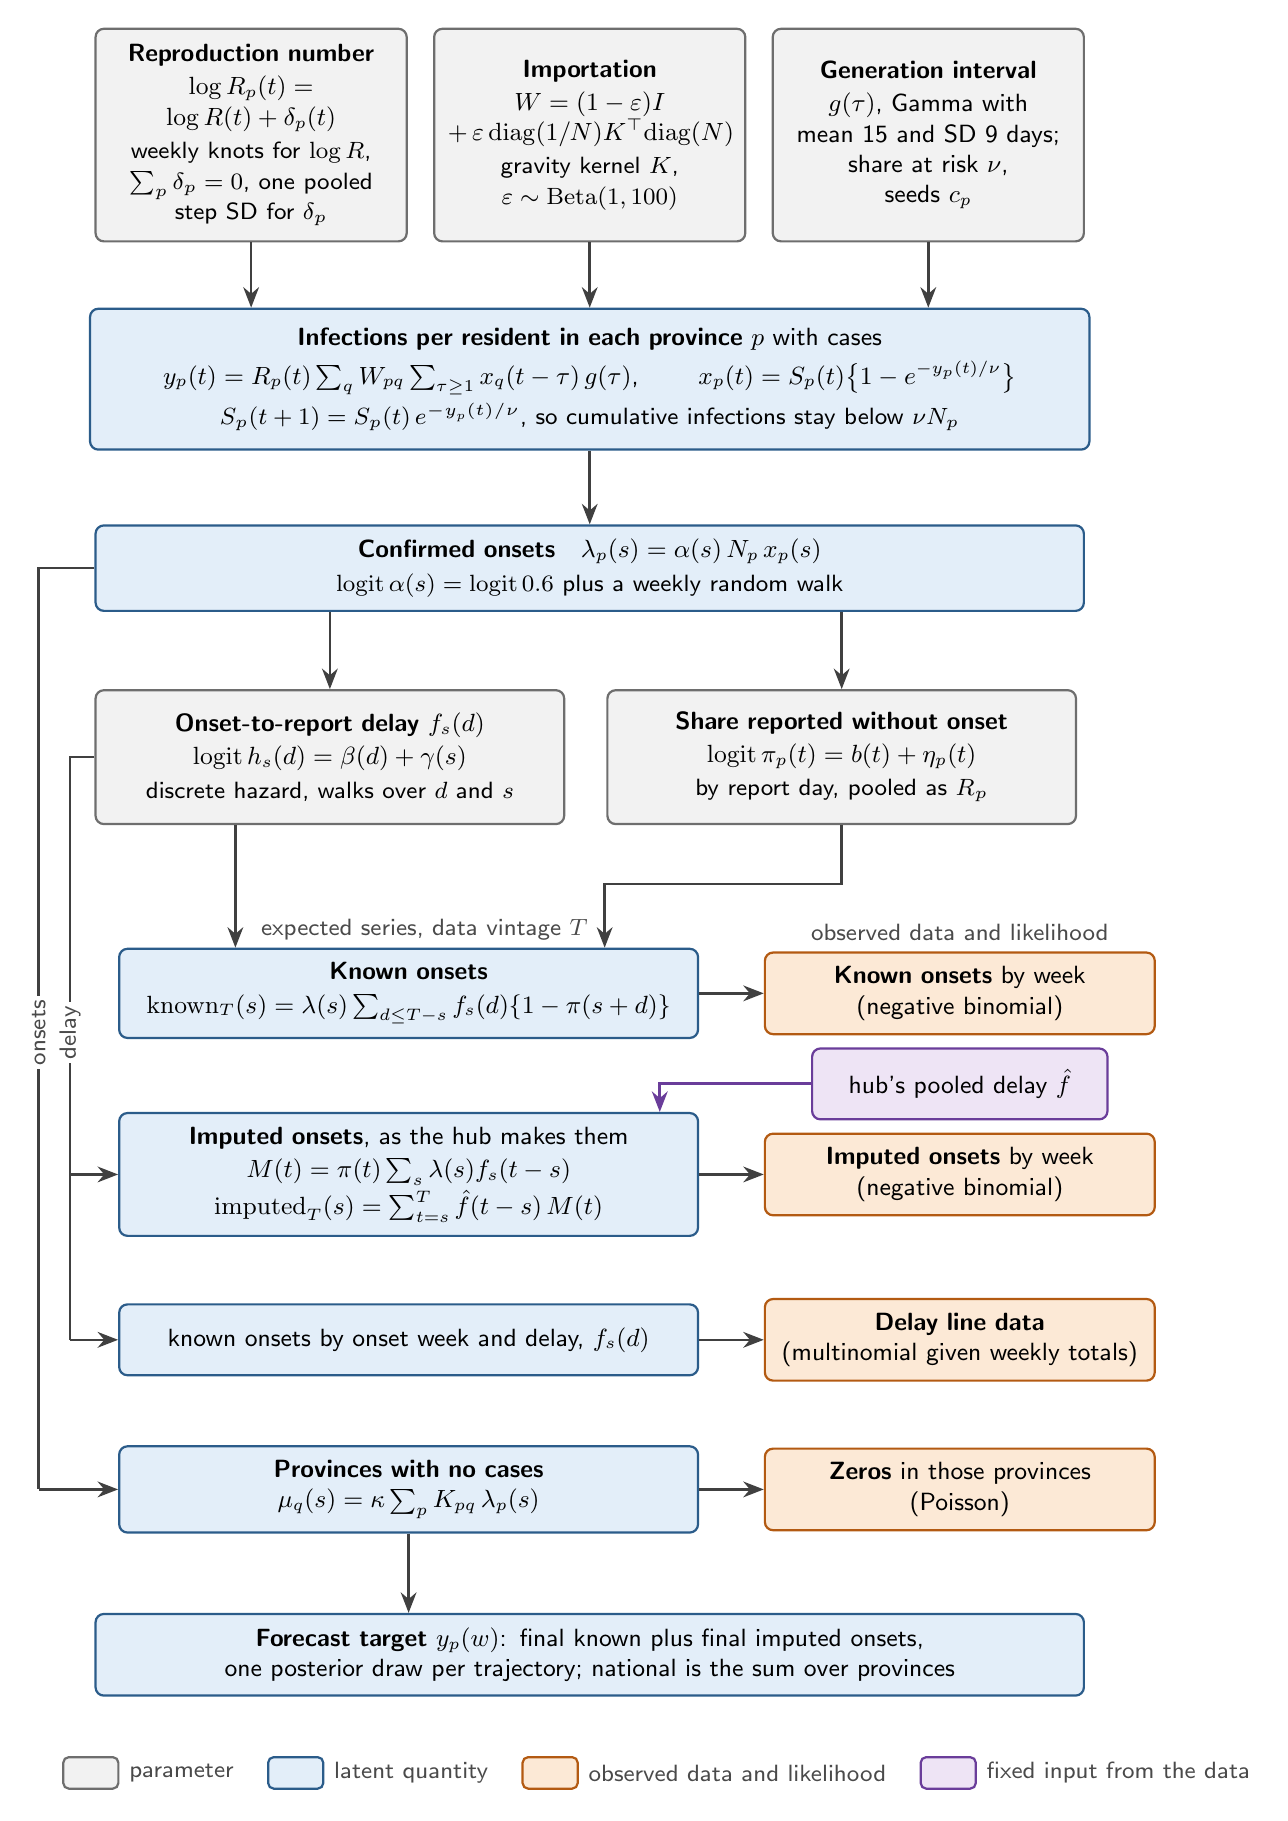
\begin{tikzpicture}[x=1cm,y=1cm]

\def\xl{-2.6}
\def\xr{4.4}
\def\wl{7.0cm}
\def\wr{4.6cm}

% ---- Parameters ----------------------------------------------------------
\node[param, text width=3.6cm, minimum height=27mm] (rt) at (-4.6,0)
  {\textbf{Reproduction number}\\[1pt]
   $\log R_p(t) = \log R(t) + \delta_p(t)$\\[1pt]
   {\footnotesize weekly knots for $\log R$,}\\ {\footnotesize $\sum_p \delta_p = 0$, one pooled}\\ {\footnotesize step SD for $\delta_p$}};
\node[param, text width=3.6cm, minimum height=27mm] (imp) at (-0.3,0)
  {\textbf{Importation}\\[1pt]
   $W = (1 - \varepsilon) I$\\ $+\, \varepsilon\, \mathrm{diag}(1/N) K^\top \mathrm{diag}(N)$\\[1pt]
   {\footnotesize gravity kernel $K$,}\\ {\footnotesize $\varepsilon \sim \mathrm{Beta}(1, 100)$}};
\node[param, text width=3.6cm, minimum height=27mm] (gi) at (4.0,0)
  {\textbf{Generation interval}\\[1pt] $g(\tau)$, Gamma with\\ mean 15 and SD 9 days;\\
   share at risk $\nu$,\\ seeds $c_p$};

% ---- Infections ----------------------------------------------------------
\node[latent, text width=12.2cm, inner sep=7pt] (inf) at (-0.3,-3.1)
  {\textbf{Infections per resident in each province} $p$ with cases\\[3pt]
   $y_p(t) = R_p(t) \sum_q W_{pq} \sum_{\tau \ge 1} x_q(t - \tau)\, g(\tau)$, \qquad
   $x_p(t) = S_p(t)\bigl\{1 - e^{-y_p(t)/\nu}\bigr\}$\\[2pt]
   {\footnotesize $S_p(t + 1) = S_p(t)\, e^{-y_p(t)/\nu}$, so cumulative infections stay below $\nu N_p$}};
\foreach \n in {rt,imp,gi}
  \draw[flow] (\n.south) -- (\n.south |- inf.north);

% ---- Confirmed onsets ----------------------------------------------------
\node[latent, text width=12.2cm] (ons) at (-0.3,-5.5)
  {\textbf{Confirmed onsets}\quad $\lambda_p(s) = \alpha(s)\, N_p\, x_p(s)$\\[1pt]
   {\footnotesize $\operatorname{logit} \alpha(s) = \operatorname{logit} 0.6$ plus a weekly random walk}};
\draw[flow] (inf.south) -- (ons.north);

% ---- Delay and missingness ----------------------------------------------
\node[param, text width=5.6cm, minimum height=17mm] (delay) at (-3.6,-7.9)
  {\textbf{Onset-to-report delay} $f_s(d)$\\[1pt]
   $\operatorname{logit} h_s(d) = \beta(d) + \gamma(s)$\\[1pt]
   {\footnotesize discrete hazard, walks over $d$ and $s$}};
\node[param, text width=5.6cm, minimum height=17mm] (miss) at (2.9,-7.9)
  {\textbf{Share reported without onset}\\[1pt]
   $\operatorname{logit} \pi_p(t) = b(t) + \eta_p(t)$\\[1pt]
   {\footnotesize by report day, pooled as $R_p$}};

% ---- Streams --------------------------------------------------------------
\def\ya{-10.9}
\def\yb{-13.2}
\def\yc{-15.3}
\def\yd{-17.2}

\node[note, anchor=south] at ({\xl+0.2},{\ya+0.55}) {expected series, data vintage $T$};
\node[note, anchor=south] at (\xr,{\ya+0.55}) {observed data and likelihood};

\node[latent, text width=\wl] (known) at (\xl,\ya)
  {\textbf{Known onsets}\\[1pt]
   $\mathrm{known}_T(s) = \lambda(s) \sum_{d \le T - s} f_s(d)\{1 - \pi(s + d)\}$};
\node[latent, text width=\wl] (imput) at (\xl,\yb)
  {\textbf{Imputed onsets}, as the hub makes them\\[1pt]
   $M(t) = \pi(t) \sum_s \lambda(s) f_s(t - s)$\\[1pt]
   $\mathrm{imputed}_T(s) = \sum_{t = s}^{T} \hat f(t - s)\, M(t)$};
\node[latent, text width=\wl] (dl) at (\xl,\yc)
  {known onsets by onset week and delay, $f_s(d)$};
\node[latent, text width=\wl] (idle) at (\xl,\yd)
  {\textbf{Provinces with no cases}\quad $\mu_q(s) = \kappa \sum_p K_{pq}\, \lambda_p(s)$};

\node[joint, text width=3.4cm] (hubf) at (\xr,{(\ya+\yb)/2})
  {hub's pooled delay $\hat f$};
\draw[jointflow] (hubf.west) -| ([xshift=-0.5cm]imput.north east);

\node[data, text width=\wr] (d_known) at (\xr,\ya)
  {\textbf{Known onsets} by week\\ (negative binomial)};
\node[data, text width=\wr] (d_imput) at (\xr,\yb)
  {\textbf{Imputed onsets} by week\\ (negative binomial)};
\node[data, text width=\wr] (d_dl) at (\xr,\yc)
  {\textbf{Delay line data}\\ (multinomial given weekly totals)};
\node[data, text width=\wr] (d_idle) at (\xr,\yd)
  {\textbf{Zeros} in those provinces\\ (Poisson)};

\foreach \a in {known,imput,dl,idle}
  \draw[flow] (\a) -- (d_\a);

% Onsets feed the delay stage; delay and missingness feed the streams.
\draw[flow] (ons.south -| delay.north) -- (delay.north);
\draw[flow] (ons.south -| miss.north) -- (miss.north);
\draw[flow] ([xshift=-1.2cm]delay.south) -- ([xshift=-1.2cm]delay.south |- known.north);
\draw[flow] (miss.south) -- ++(0,-0.75) -| ([xshift=-1.2cm]known.north east);
% Trunks on the left for the streams below the first.
\def\bt{-6.9}
\draw[line width=0.9pt, draw=black!75] (delay.west) -- (\bt,0 |- delay.west) -- (\bt,\yc);
\draw[flow] (\bt,\yb) -- (imput.west);
\draw[flow] (\bt,\yc) -- (dl.west);
\def\bo{-7.3}
\draw[line width=0.9pt, draw=black!75] (ons.west) -- (\bo,0 |- ons.west) -- (\bo,\yd);
\draw[flow] (\bo,\yd) -- (idle.west);
\node[edgelabel, rotate=90] at (\bt,{\ya-0.5}) {delay};
\node[edgelabel, rotate=90] at (\bo,{\ya-0.5}) {onsets};

% ---- Forecast ------------------------------------------------------------
\node[latent, text width=12.2cm] (fc) at (-0.3,{\yd-2.1})
  {\textbf{Forecast target} $y_p(w)$: final known plus final imputed onsets,\\
   one posterior draw per trajectory; national is the sum over provinces};
\draw[flow] (idle.south) -- (idle.south |- fc.north);

% ---- Key -------------------------------------------------------------------
\colourkey[joint]{(-7.0,{\yd-3.6})}

\end{tikzpicture}
\end{document}
